%% Haruka Nagao <karuka.nagao@ku.edu>
%% 2019-02-16 
%% Original Templates downloaded from https://gitlab.crmda.ku.edu/crmda/tikz
%%

\documentclass[border=50pt]{standalone}

\usepackage{tikz}

\tikzstyle{ov}=[shape=rectangle,
                draw=black!80,
                minimum height=0.6cm,
                minimum width=0.6cm,
                thick]
                
\tikzstyle{av}=[shape=rectangle,
                draw=black!80,
                fill=black!10,
                minimum height=0.6cm,
                minimum width=0.6cm,
                thick]

\tikzstyle{lv}=[shape=circle,
                draw=black!80,
                thick,
                minimum width=1cm]

\begin{document}

%% ">=stealth" sets the arrow head style
%% "semithick" sets the line width (0.6 pt)
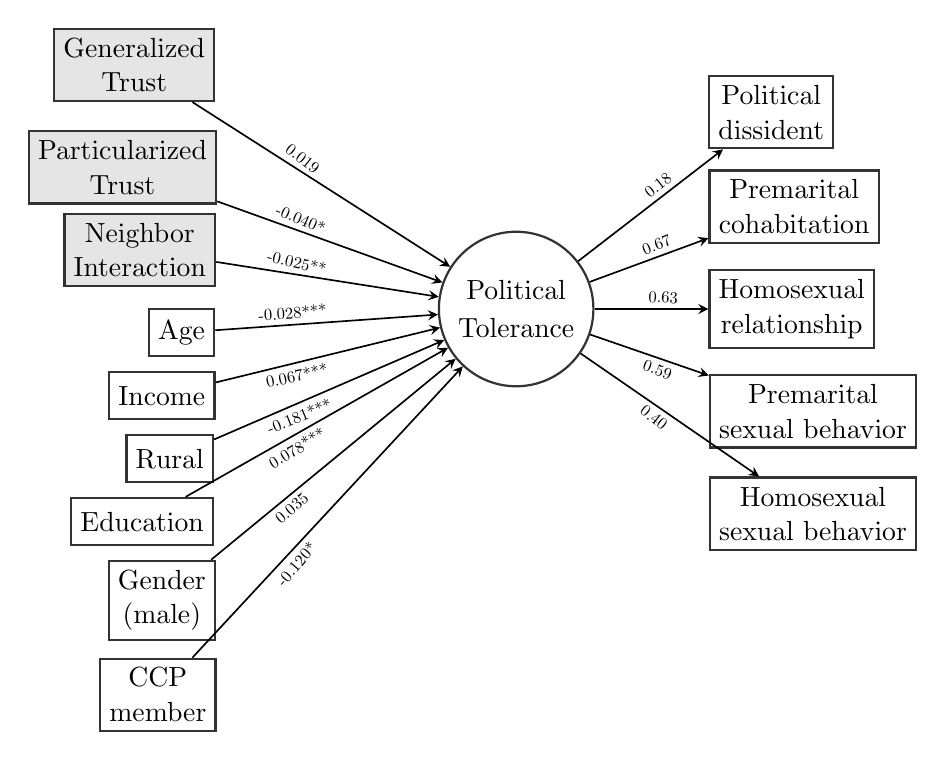
\begin{tikzpicture}[>=stealth,semithick]

% dependent variable
\node[lv, align=center] (y1) at (0, -1) {Political \\[0.2em]{Tolerance}};

% independent variables
\node[av, align=center] (x1) at (-4.85, 2.1) {Generalized \\[0.05em]{Trust}};
\node[av, align=center] (x2) at (-5, 0.8) {Particularized \\[0.05em]{Trust}};
\node[av, align=center] (x3) at (-4.78, -0.25) {Neighbor \\[0.05em]{Interaction}};
\node[ov] (x4) at (-4.25, -1.3) {Age};
\node[ov] (x5) at (-4.5, -2.1) {Income};
\node[ov] (x6) at (-4.4, -2.9) {Rural};
\node[ov] (x7) at (-4.75, -3.7) {Education};
\node[ov, align=center] (x8) at (-4.5, -4.7) {Gender\\[0.05em]{(male)}};
\node[ov, align=center] (x9) at (-4.55, -5.9) {CCP \\[0.05em]{member}};


% latent variables
\node[ov, align=center] (f1) at (3.24, 1.5)  {Political \\[0.05em]{dissident}};
\node[ov, align=center] (f2) at (3.53, 0.3)  {Premarital \\[0.05em]{cohabitation}};
\node[ov, align=center] (f3) at (3.5, -1)  {Homosexual \\[0.05em]{relationship}};
\node[ov, align=center] (f4) at (3.77, -2.3)  {Premarital \\[0.05em]{sexual behavior}};
\node[ov, align=center] (f5) at (3.77, -3.6)  {Homosexual \\[0.05em]{sexual behavior}};

% paths
\path[->] (y1) edge node[above,scale=0.6, pos=0.6, rotate=38] {0.18} (f1)
          (y1) edge node[above,scale=0.6, pos=0.6,rotate=22] {0.67} (f2)
          (y1) edge node[above,scale=0.6,pos=0.6, rotate=-2] {0.63} (f3)
          (y1) edge node[below,scale=0.6,pos=0.6, rotate=-20] {0.59} (f4)
          (y1) edge node[below,scale=0.6, pos=0.45,rotate=-38] {0.40} (f5);
          
\path[->] (x1) edge node[above, pos=0.4, scale=0.6, rotate=-38] {0.019} (y1)
          (x2) edge node[above, pos=0.35,scale=0.6, rotate=-23] {-0.040*} (y1)
          (x3) edge node[above, pos=0.35,scale=0.6, rotate=-13] {-0.025**} (y1)
          (x4) edge node[above, pos=0.35,scale=0.6, rotate=4] {-0.028***} (y1)
          (x5) edge node[below, pos=0.35,scale=0.6, rotate=12] {0.067***} (y1)
          (x6) edge node[below, pos=0.35,scale=0.6, rotate=22] {-0.181***} (y1)
          (x7) edge node[below, pos=0.4,scale=0.6, rotate=31] {0.078***} (y1)
          (x8) edge node[below, pos=0.3,scale=0.6, rotate=40] {0.035} (y1)
          (x9) edge node[below, pos=0.35,scale=0.6, rotate=49] {-0.120*} (y1);
\end{tikzpicture}


\end{document}
